\documentclass[]{nthu_thesis}

% set proper margins
\geometry{
  a4paper,
  left=3cm,
  right=3cm,
  top=3cm,
  bottom=3cm,
  bindingoffset=0mm,
  headheight=0pt,
  headsep=0pt,
  footskip=18pt
}
\setlength{\hoffset}{0pt}
\setlength{\oddsidemargin}{15.5pt}
\setlength{\marginparwidth}{0pt}
\setlength{\marginparsep}{0pt}


\begin{document}
\pagestyle{plain} %This is the default style for most document classes. It places the page number centered in the footer, with an empty header.

%%% Necessary fields for this thesis data %%%
% Add your custom class definitions here if any

\newcommand{\degreeZH}{碩}  % 畢業學位，碩 for masters 或 博 for PHD
\newcommand{\degreeEN}{Master's Thesis}  %  Fill in your degree "Master's Thisis" for masters 或 "Doctoral Dissertation" for PHD
\newcommand{\titleZH}{這裡填入論文中文題名} % 此括弧內填入論文中文標題Chinese title here
\newcommand{\titleEN}{Type English Title Here} % 此括弧內填入論文英文標題
\newcommand{\instituteZH}{學系班} % 此括弧內填入畢業生所屬學系班
\newcommand{\instituteEN}{Grad. Prog.} % Graduation Dept./Inst. Name
\newcommand{\studentID}{110011000} %填入畢業生的學號 your student ID
\newcommand{\studentZH}{王大明} % 此括弧內填入畢業生的中文名字 Graduate's Chinese Name here
\newcommand{\studentEN}{Da-Ming Wang} %此括弧內填入畢業生的英文姓名 Graduate's Eng. Name here
\newcommand{\advisorZH}{楊振寧} %此括弧內填入指導教授的中文名字，如有兩個，請自行增加
\newcommand{\advisorEN}{David Yang} % 此括弧內填入 advisor's English Name
\newcommand{\yearZH}{114} %此括弧內填入畢業年(民國) Year of ROC  ，就是口試日期的那個月
\newcommand{\monthZH}{6} % Graduation (Oral exam) month of ROC 
\newcommand{\yearEN}{2025} % Graduation (oral exam) Year  
\newcommand{\monthEN}{June} % Graduation (oral Exam) month


\begin{titlepage}

\newgeometry{a4paper,left=2.54cm,right=3.18cm,top=3.18cm,bottom=2.54cm} % 根據清大註冊組 封頁 (only)格式

\begin{spacing}{1.3}  
     \begin{center}
       \fontsize{24pt}{28pt}\selectfont
        國\hspace{1em}立\hspace{1em}清\hspace{1em}華\hspace{1em}大\hspace{1em}學\\
        National Tsing Hua University\\
        \vspace{1.0 cm}
        \degreeZH~~~士~~~論~~~文\\
        \degreeEN 
   
    \vspace{2em}  %for controlling veretical space
    \Huge
        \titleZH\\
    \titleEN \\
    \vspace{3em} %for controlling veretical space
    
   \Large

  %\leftskip 1.0cm
%  \setlength\tabcolsep{3pt} % default: 6pt
\renewcommand{\arraystretch}{1.3} % default value is 1.0
      \begin{tabular}{ l }  %l: Left-aligned column.
        系所別：~\instituteZH\\
        Dept.~/~Grad. Inst.:\hspace{0.5em}\instituteEN\\
        學號~ Student ID:\hspace{0.5em}\studentID\\
        研究生~Author：\hspace{0.5em}\studentZH\hspace{0.5em}\studentEN\\
        指導教授~Advisor：\hspace{0.5em}\advisorZH\hspace{0.5em}\advisorEN
    \end{tabular}\\
    
   \vspace{3em} 
           
    中~~華~~民~~國~~\zhdigits{\yearZH}~年~~\zhdigits{\monthZH}~月\\
    \monthEN~\yearEN
     \end{center}
\end{spacing}
  \restoregeometry
\end{titlepage}



%intentionally to add a blank page 
\newpage
\null
\thispagestyle{empty}
\newpage

% 書名頁
\begin{titlepage}

\newgeometry{a4paper,left=2.54cm,right=3.18cm,top=3.18cm,bottom=2.54cm} % 根據清大註冊組 封頁 (only)格式

\begin{spacing}{1.3}  
     \begin{center}
       \fontsize{24pt}{28pt}\selectfont
        國\hspace{1em}立\hspace{1em}清\hspace{1em}華\hspace{1em}大\hspace{1em}學\\
        National Tsing Hua University\\
        \vspace{1.0 cm}
        \degreeZH~~~士~~~論~~~文\\
        \degreeEN 
   
    \vspace{2em}  %for controlling veretical space
    \Huge
        \titleZH\\
    \titleEN \\
    \vspace{3em} %for controlling veretical space
    
   \Large

  %\leftskip 1.0cm
%  \setlength\tabcolsep{3pt} % default: 6pt
\renewcommand{\arraystretch}{1.3} % default value is 1.0
      \begin{tabular}{ l }  %l: Left-aligned column.
        系所別：~\instituteZH\\
        Dept.~/~Grad. Inst.:\hspace{0.5em}\instituteEN\\
        學號~ Student ID:\hspace{0.5em}\studentID\\
        研究生~Author：\hspace{0.5em}\studentZH\hspace{0.5em}\studentEN\\
        指導教授~Advisor：\hspace{0.5em}\advisorZH\hspace{0.5em}\advisorEN
    \end{tabular}\\
    
   \vspace{3em} 
           
    中~~華~~民~~國~~\zhdigits{\yearZH}~年~~\zhdigits{\monthZH}~月\\
    \monthEN~\yearEN
     \end{center}
\end{spacing}
  \restoregeometry
\end{titlepage}



 \let\cleardoublepage=\clearpage % Place this after \end{titlepage} for removing the blank page 
 
%\restoregeometry  %back to NTHU required geometry setting


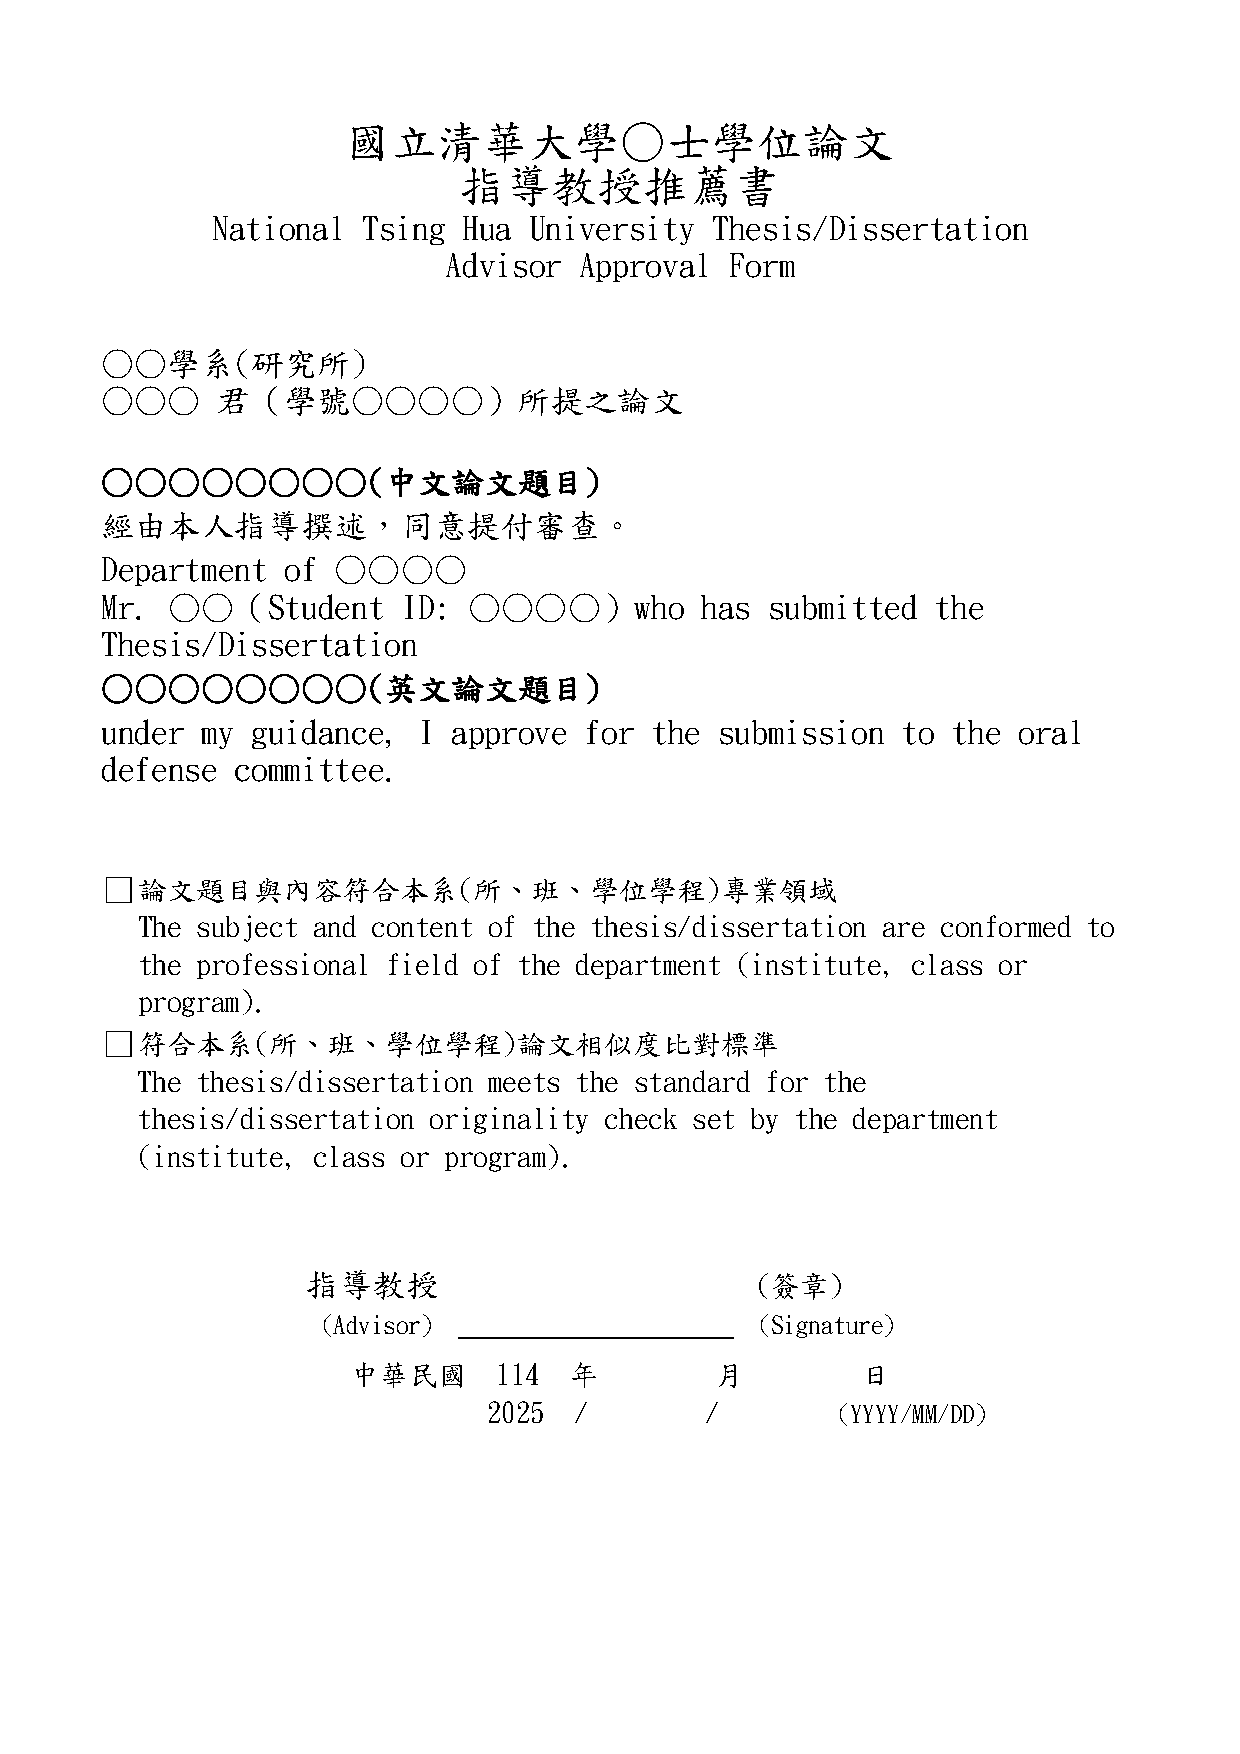
\includepdf[pages=1, angle=0, fitpaper=true,
    keepaspectratio, pagecommand={{\thispagestyle{empty}}},offset=-0.0cm 0.0cm]{./front/Advisor Approval Form.pdf}

%\cftaddtitleline{<ext>}{<kind>}{<text>}{<page>} intead of using \addcontentsline command  for without page numbering

\cftaddtitleline{toc}{chapter}{指導教授推薦書}{}

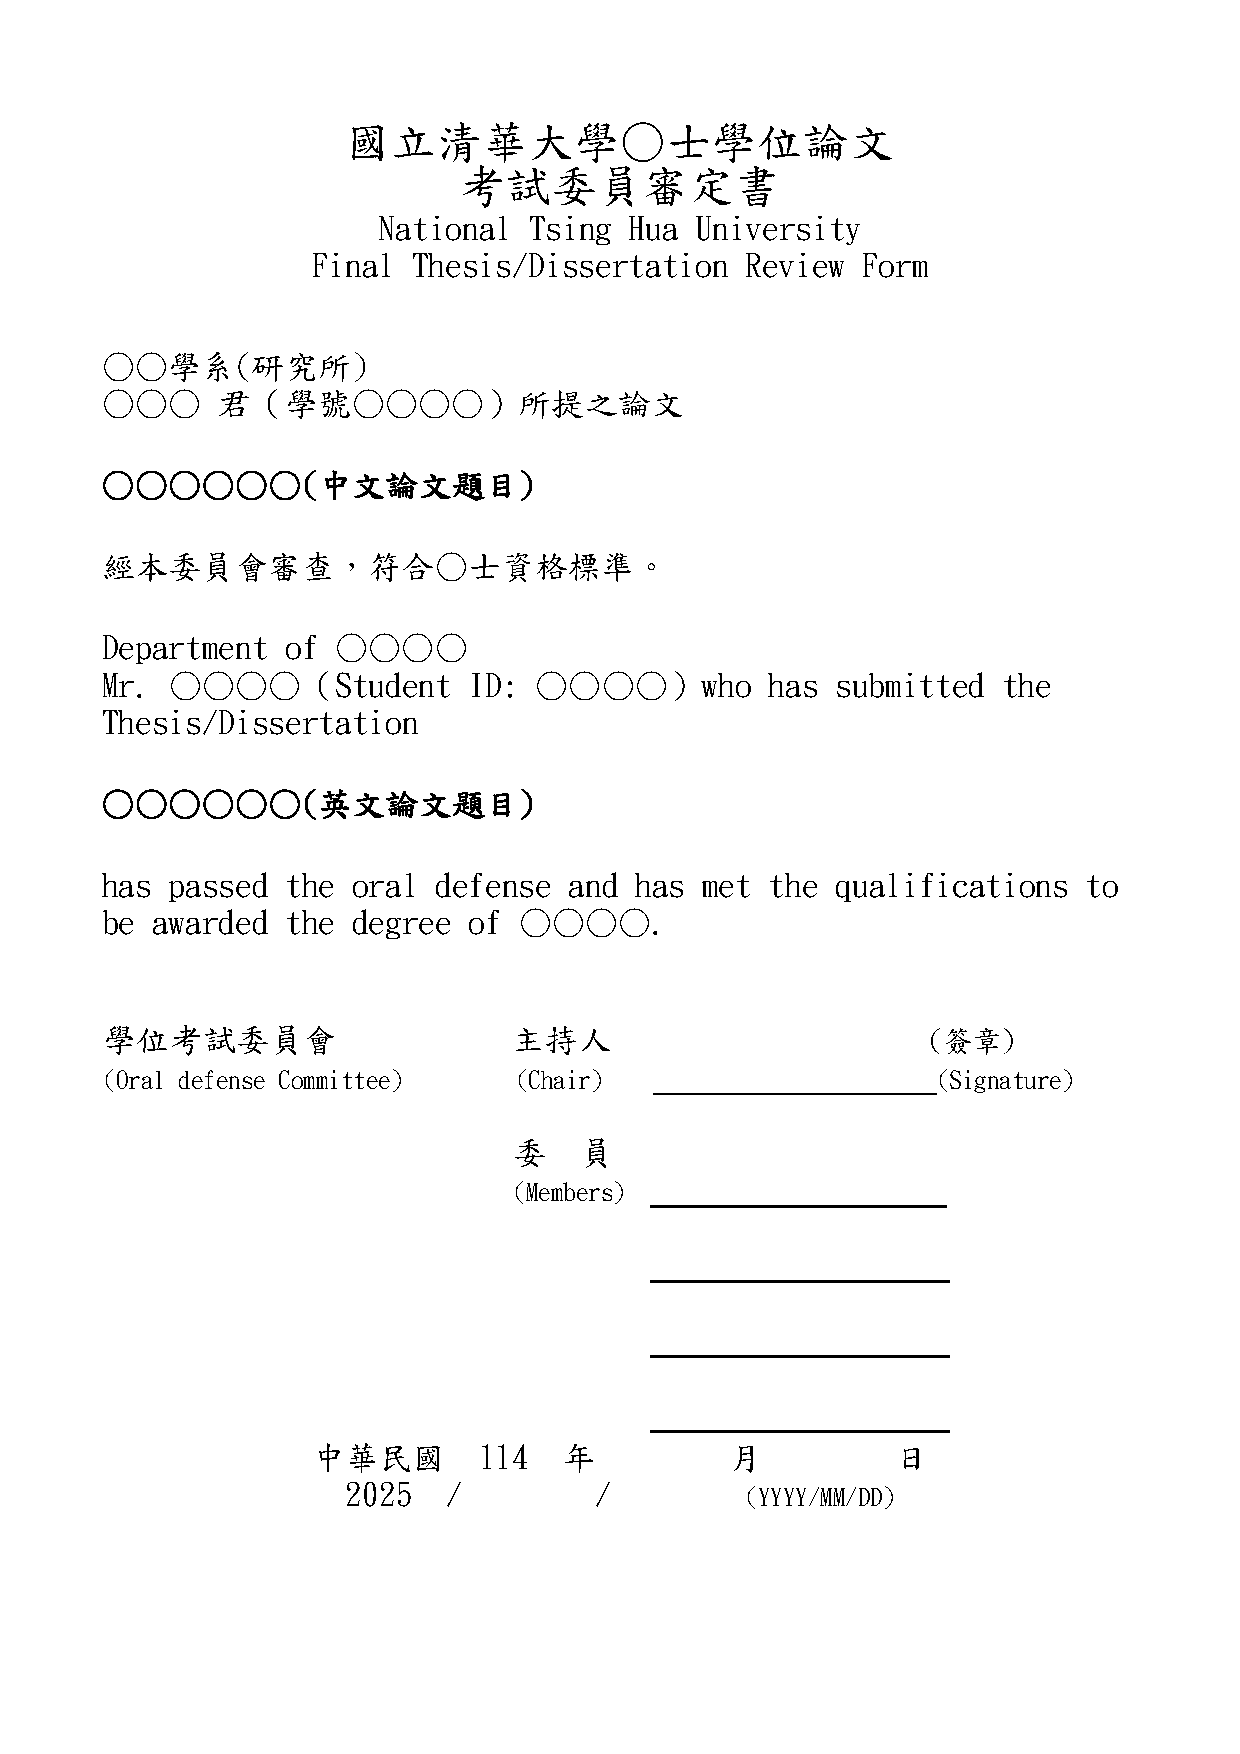
\includepdf[pages=1, angle=0, fitpaper=true,
       keepaspectratio, pagecommand={{\thispagestyle{empty}}},offset=-0.0cm 0.0cm]{./front/Thesis Review Form.pdf} %offset=+right +up

\cftaddtitleline{toc}{chapter}{考試委員審定書}{}

\frontmatter %Use for book class 

%%% Necessary 中文摘要%%%
\chapter*{摘要}
\addcontentsline{toc}{chapter}{摘要}
	摘要是整篇論文的濃縮總結，需精簡扼要，涵蓋論文核心內容，邏輯連貫地總結各章節要點，吸引讀者興趣。建議控制在一頁內，約400–600字，避免使用圖表。
    
\textbf{內容要素：}
\begin{itemize}
    \item 研究動機與目標：闡述研究背景、核心問題及主要目標。
    \item 研究範圍：明確界定研究的課題與範疇。
    \item 研究方法：概述方法、技術或工具，並簡述其合理性。
    \item 主要結果：突出核心發現或數據。
    \item 結果比較與意義：將結果與研究目標及文獻比較，凸顯貢獻。
    \item 未來影響與建議：說明研究對學術或實務的助益，提出未來方向。
\end{itemize}

\textbf{撰寫建議：}
\begin{itemize}
    \item 使用精煉語言，確保非領域專家也能理解。
    \item 完成論文其他部分後再提煉摘要，確保內容全面。
    \item 使用純文字格式（無HTML或特殊格式），便於圖書館建檔與網路檢索。
    \item 附上5–7個關鍵詞，提升論文檢索率。
\end{itemize}

\medskip
\textbf{關鍵字：}論文格式、圖書館建檔、範例、提煉、圖書館建檔
       % 插入中文摘要於此 Insert Chinese Abstract
%\setcounter{page}{1}  %set page begins with i
\clearpage

\chapter*{Abstract}
\addcontentsline{toc}{chapter}{Abstract}
	The abstract is a concise summary of the dissertation, encapsulating its core content in a clear, logically coherent manner to engage readers. It should be limited to one page, approximately 300–500 words, and avoid including figures or tables.
    
\textbf{Content Elements:}
\begin{itemize}
    \item Research Motivation and Objectives: Describe the background, core research question, and primary goals.
    \item Research Scope: Clearly define the topics and boundaries of the study.
    \item Methodology: Summarize the methods, techniques, or tools used and briefly justify their selection.
    \item Key Results: Highlight the most significant findings or data.
    \item Comparison and Significance: Compare results with the initial objectives and existing literature, emphasizing contributions.
    \item Impact and Future Directions: Discuss the study’s benefits to academic or practical fields and suggest future research or applications.
\end{itemize}


\textbf{Writing Tips:}
\begin{itemize}
    \item Use precise, accessible language to ensure clarity for non-experts.
    \item Draft the abstract after completing other sections to ensure it fully reflects the dissertation’s content.
    \item Format in plain text (no HTML or special formatting) to comply with library archiving and online search requirements.
\end{itemize}

\medskip
\textbf{Keywords:} database, HTML, library archiving, dissertation, methodology       % 插入英文摘要於此 Insert English Abstract
\clearpage


%\pagenumbering{roman} %set lowercase Roman numerals for page numbers if set article class
\chapter*{致謝}
\addcontentsline{toc}{chapter}{致謝}
致謝用於表達對研究與論文完成過程中提供支持者的感謝，展現學術禮儀與個人感恩。

\textbf{內容要素：}
\begin{itemize}
    \item 感謝間接貢獻者，如資助機構、提供設備的單位、參與討論的學者或同儕。
    \item 感謝研究執行協助者，如實驗室助理、技術人員或同學。
   \item 可感謝對研究生涯或個人成長的支持者，如父母、家人或朋友。
\end{itemize}

\bigskip
\textbf{撰寫建議：}
\begin{itemize}
   \item 語氣真誠且適度個人化，保持簡潔與專業，避免過於冗長或情感化。
   \item 按貢獻重要性排序，先謝指導教授與資助單位，再提及個人支持者。
   \item 確保不遺漏重要貢獻者，但無需逐一列出所有相關人士。

\end{itemize}


       % 致謝（Acknowledgement）
\clearpage

% 生成目錄與符號列表
% generate Contents of Tables, lists of figures, tables, 
\renewcommand*\contentsname{目次}
\pagestyle{plain}
\tableofcontents
\addcontentsline{toc}{chapter}{目次}
\clearpage

\renewcommand*\listfigurename{圖次}
\listoffigures  % Insert list of figures
\addcontentsline{toc}{chapter}{圖次}
\clearpage

\renewcommand*\listtablename{表次}
\listoftables  % Insert list of tables
\addcontentsline{toc}{chapter}{表次}
\clearpage

% Nomenclature (optional). List unfamiliar terms, symbols, acronyms and their meanings. Delete if not needed

%vNomenclature (optional). List unfamiliar terms, symbols, acronyms and their meanings.

\nomenclature{\(c\)}{Speed of light in a vacuum}
\nomenclature{\(h\)}{Planck constant}


%\renewcommand{\nomname}{List of Symbols}
\renewcommand{\nomname}{符號列表}  %needed for Chinese version
\printnomenclature    % if needed 符號列表（Nomenclature）
\addcontentsline{toc}{chapter}{符號列表}
\clearpage


% 論文內容Contents of Thesis

\mainmatter  %for book class only
%\pagenumbering{arabic} % already default for book class, Arabic/Indic page numbers, needed for article class

\pagestyle{plain} % This is the default style for most document classes. It places the page number centered in the footer, with an empty header.
\chapter{Introduction}

\section{Background and Motivation}

Accurate force generation and measurement at pico- to nano-Newton levels are essential for probing living cells and monitoring active biological processes in aqueous solution. For this class of application, force precision alone is not sufficient. A practical system must also maintain stable high-speed operation, suppress channel interaction, and provide repeatable closed-loop behavior.

Scanning-probe-based technologies have enabled major progress in mechanobiology. Atomic force microscopy provides high-resolution force sensing and topography measurement, but practical throughput can become limited when dense three-dimensional probing is required over samples with large topographic variation.

Optical trapping is another powerful approach for micro-scale manipulation in fluidic environments. However, its practical deployment may face constraints in probe specificity, operational robustness, and sustained force authority under experimental conditions relevant to long-duration biological studies.

Magnetic actuation is attractive in this context because it enables remote, non-contact force generation with low optical burden. A Hall-sensor-based hexapole electromagnetic actuator extends this capability to three-dimensional force production in an over-actuated architecture. Prior studies have already established strong technical baselines, including current-based and flux-based allocation frameworks, high-bandwidth flux regulation, and pico-Newton-level force control.

The remaining need is therefore not another demonstration that high performance is possible. The key need is to explain why the achieved performance is physically and systematically justified. In this dissertation, the central motivation is to make the design rationale explicit: what tradeoffs are made, what physical issue each step addresses, and how each effect is verified.

This motivation starts from open-loop calibration of magnetic flux generation in the hexapole actuator. The measured responses indicate channel coupling, uncertainties caused by magnetic remanence and hysteresis, and frequency-dependent deviations in both magnitude and phase. These observed deviations affect the consistency between commanded and realized flux dynamics and can propagate to force-generation error if they are not explicitly addressed in the control design.

Guided by these observations, this dissertation adopts a linked investigation from system identification to flux control and force generation. The intended outcome is a traceable and reproducible decision path that explains how performance is obtained and how the framework can be extended with confidence for ultra-precise high-speed untethered manipulation in aqueous solution.

In this thesis, the primary emphasis is the stepwise decomposition of this control chain and the physical interpretation of each design decision. Workflow reproducibility and process structuring are treated as supporting contributions that strengthen implementation and reuse.

\section{Research Objective and Scope}

The objective of this dissertation is to establish a traceable control-oriented framework for Hall-sensor-based hexapole actuation, and to show how design decisions propagate from model construction to final force behavior. The scope focuses on control-system design, analysis, and validation for magnetic manipulation in aqueous solution.

\textbf{Aim 1: System identification for control use.}
This aim establishes an identification workflow that converts open-loop physical observations into model information suitable for controller design. The key question is how coupling, hysteresis-related behavior, and dynamic characteristics should be represented for design decisions. Simulation and experimental evidence are presented together in the same thread to evaluate both model consistency and control relevance.

\textbf{Aim 2: Flux-control design and tradeoff analysis.}
This aim studies inner-loop flux control from a design-tradeoff perspective, including baseline PI control and model-based control structures. The key question is which controller element addresses which physical issue and how this affects multi-axis decoupling quality. Simulation and experimental results are reported together to show where prediction and measured behavior agree or diverge, and why.

\textbf{Aim 3: Force-generation quality analysis.}
This aim examines the force-generation chain with emphasis on decoupling behavior, scheduling effects, and force-quality indicators. The key question is how upstream design choices constrain downstream force output quality. Simulation and experimental results are presented together within this thread rather than separated into a standalone result-only section.

Across the three aims, the primary contribution is the explicit explanation of design tradeoffs through a traceable and physically interpretable decision path. Workflow integration, automation, and process reproducibility are supporting contributions. Claims are made under tested operating conditions, and broad biological interpretation is outside the scope of this dissertation.

\section{Dissertation Overview}

This dissertation is organized as follows. Chapter 1 introduces the background, motivation, objective, scope, and the three technical aims.

Chapter 2 presents the full system overview, including the hexapole actuation platform, sensing and force-production chain, layered control architecture, and the shared analysis framework used throughout this thesis.

Chapter 3 develops the system-identification thread and explains how open-loop observations are converted into model information for control design. Simulation and experimental analyses are presented together in the same technical context.

Chapter 4 presents the flux-control thread, including baseline and model-based designs, component-level interpretation, and multi-axis decoupling behavior. Simulation and experimental evidence are discussed together for direct comparison with design intent.

Chapter 5 presents the force-generation thread and analyzes how allocation and scheduling choices influence force quality and cross-axis behavior. The chapter also integrates cross-layer validation and closes with concluding remarks and future directions.

Together, Chapters 3 through 5 provide one continuous evidence chain from observed actuator behavior to model choice, controller design, and final force-output quality.

% !TeX root = ../main.tex

\chapter{System Overview and Unified Development Framework}

\section{Hexapole Actuation Platform}

This dissertation considers a Hall-sensor-based hexapole electromagnetic actuator for precision manipulation in aqueous solution. The platform uses six independently driven poles to generate magnetic flux and magnetic-field gradients in a three-dimensional workspace. Because force objectives are three-dimensional while actuation is six-dimensional, the system is over-actuated and requires explicit allocation and control logic.

From an engineering perspective, the platform combines non-contact operation, strong force authority, and microscope compatibility. These properties make it suitable for high-speed untethered manipulation when flux generation and multi-axis interaction are properly handled.

\section{End-to-End Control Chain}

The physical and computational chain considered in this work starts from actuation commands, proceeds through magnetic-flux generation, and ends at force output on the probe. Hall-sensor measurements provide the core feedback channel for closed-loop flux regulation, and the force-generation stage maps control outputs to task-level force behavior.

For dissertation-level reasoning, this chain is treated as one connected pipeline rather than isolated blocks. Upstream uncertainty and design decisions can propagate to downstream force quality, so each stage must be interpreted in relation to the full chain.

\section{Development-Process Structuring Blueprint (Pillar A)}

The first equal-weight pillar is process structuring. Chapter 2 defines a reusable blueprint for developing hexapole-form tweezers:

1. establish platform and measurement context;
2. extract control-use model information from calibration data;
3. design and validate flux-control structure;
4. evaluate force-generation quality under design choices;
5. close the chain with cross-layer interpretation.

This blueprint makes stage boundaries explicit and keeps design decisions traceable from observation to final force behavior.

\section{Workflow Automation Interfaces (Pillar B)}

The second equal-weight pillar is workflow automation. Chapter 2 defines where automation is integrated into the blueprint:

1. identification-stage repeatable processing and fitting flow;
2. control-stage simulation-and-tuning loop after identification;
3. stage-to-stage data handoff for force-generation validation.

These interfaces are defined to reduce development burden and improve reproducibility when deploying the framework on additional hexapole-form platforms.

\section{Chapter Interface to Chapters 3--5}

Chapter 2 provides the common language and unified framework for the remaining technical chapters. Chapter 3 develops the identification thread, Chapter 4 develops the flux-control thread, and Chapter 5 develops the force-generation thread and closes the cross-layer evidence chain.

\chapter{System Identification of Hexapole Magnetic Flux Dynamics}

\section{Chapter Objective and Evidence Contract}

This chapter develops the system-identification stage of the thesis workflow. The objective is to convert open-loop observations into model information that is directly usable for control design and downstream force-generation analysis. The evidence contract of this chapter is to present simulation and experimental results in the same thread, so model quality is assessed by control relevance rather than by fitting score alone.

\section{Open-Loop Calibration Context and Data Interface}

This section defines the calibration context used in this dissertation, including excitation protocol, measurement channels, operating conditions, and data acquisition interface. The purpose is to make the identification input reproducible and to clarify what uncertainty sources are present before controller design begins.

\section{Frequency-Response Construction and Observable Phenomena}

This section describes how frequency-domain information is constructed from calibration data and how key physical phenomena are interpreted at this stage, including coupling behavior, remanence- and hysteresis-related effects, and frequency-dependent response variation. The focus is on observable evidence and its relevance to model structure selection.

\section{Control-Use Model Structure and Reduction Logic}

This section presents the model representation used for control development and the reduction logic that maps detailed channel behavior into a controller-usable form. The objective is to preserve physically meaningful coupling information while keeping a practical interface for the control-design stage.

\section{Fitting Strategy and Control-Relevant Quality Criteria}

This section defines the fitting strategy and quality criteria used in identification, with emphasis on low-frequency control relevance and predictable downstream behavior. The criteria are organized to support later design decisions in flux control and force generation.

\section{Simulation and Experimental Validation}

This section provides paired simulation and experimental validation for the identification stage. The reported results verify consistency between modeled behavior and measured behavior under tested operating conditions, and establish the handoff artifacts required by Chapter 4.

\section{Chapter Summary and Interface to Chapter 4}

This chapter concludes by summarizing what model information is accepted for control design, what uncertainty remains, and how identification outputs are passed to the flux-control stage. This closes the first link of the ID-to-Flux-to-Force evidence chain.

\chapter{Flux Control Design and Validation}

\section{Chapter Objective and Interface from Identification}

This chapter develops the flux-control stage based on the control-use model obtained in Chapter 3. The objective is to translate identified dynamics into practical controller design and to quantify how design choices affect bandwidth, decoupling behavior, and robustness under tested operating conditions.

\section{Flux-Control Problem Definition and Design Targets}

This section defines the inner-loop control problem, including tracking objective, decoupling requirement, disturbance sensitivity, and target dynamic behavior. These targets provide a common basis for comparing controller structures in the rest of this chapter.

\section{Baseline PI Control Design and Initial Validation}

This section presents the baseline PI design path and its expected behavior from model-based prediction. Simulation and experimental results are used together to identify where baseline design is sufficient and where performance limitations emerge.

\section{Model-Based Control with Disturbance Rejection}

This section develops the model-based control structure, including disturbance-rejection elements and design parameters that shape closed-loop behavior. The emphasis is on design rationale, not only performance display, so each control component is linked to a specific physical issue.

\section{Component-Level Interpretation and Decoupling Analysis}

This section compares controller structures at component level and interprets their effects on coupling suppression, tracking behavior, and sensitivity to model mismatch. The analysis provides the causal link required for downstream force-generation interpretation.

\section{Simulation and Experimental Validation}

This section provides paired simulation and experimental validation across representative test conditions. The results show where predicted and measured behavior are consistent and establish the validated controller outputs that will be consumed by Chapter 5.

\section{Chapter Summary and Interface to Chapter 5}

This chapter concludes with the accepted flux-control configuration and its validated behavior envelope. It then defines the interface handoff to the force-generation stage, including which outputs are treated as trusted inputs for force-quality analysis.

\chapter{Force Generation, Motion Control, and Conclusions}

\section{Chapter Objective and Interface from Flux Control}

This chapter develops the force-generation and motion-control stages using validated outputs from the flux-control stage. The objective is to evaluate how upstream identification and control decisions influence downstream force quality, tracking behavior, and operational outcomes in a traceable manner.

\section{Force-Generation Interface and Allocation Logic}

This section defines the force-generation interface from desired task-level force behavior to actuator-level command variables. The emphasis is on interface consistency, allocation logic, and implementation assumptions required for reproducible operation.

\section{Force- and Motion-Quality Criteria and Scheduling Context}

This section defines force- and motion-quality criteria used in this dissertation, including main-axis quality, cross-axis interaction behavior, tracking-level behavior, and scheduling-related response characteristics. The criteria are selected to support control-oriented interpretation and chapter-to-chapter comparability.

\section{Simulation and Experimental Validation of Force and Motion Outputs}

This section presents simulation and experimental validation in the same technical thread to assess force-generation and motion-control behavior under representative operating conditions. The goal is to verify whether force and motion output quality are consistent with the intended design chain from identification and flux control.

\section{Tracing Design Decisions from Identification to Flux, Force, and Motion Control}

This section closes the evidence chain by tracing how upstream modeling and control decisions propagate to force-level and motion-level outcomes through validated interfaces. The discussion focuses on evidence-supported links under tested conditions, and on how this traceability supports reproducible development.

\section{Conclusions and Future Directions}

This section summarizes the dissertation-level contribution as an automation-oriented and control-grounded development framework for Hall-sensor-based hexapole magnetic tweezers. It also outlines practical next steps for extending the framework in future studies while preserving traceability and reproducibility.


% 參考文獻  References

\cleardoublepage
\printbibliography[ heading=bibintoc,title={參考文獻} ]

%\addcontentsline{toc}{chapter}{參考文獻}
%\addcontentsline{toc}{chapter}{Bibliography}

% 附錄 如果沒有附錄，可以刪除這整段
% Appendices  if no appendix, this section can be deleted
\renewcommand*\appendixname{附錄}
\appendix   % Signal the start of the appendix section

\chapter*{\centering{Appendices}}
\addtocontents{toc}{\protect\contentsline {chapter}{附錄}{}{}}

% !TeX root = ../main.tex
\chapter{模型參數表}
附錄收錄輔助性質但篇幅較大的資料，增強論文完整性，不影響正文流暢性。

\section{內容要素}
\begin{itemize}
    \item 包含詳細數據表、程式碼、原始測量記錄、額外圖表、推導過程、裝置設計圖等。
   \item 每項附錄需編號並附簡短說明，與正文對應。
 
\end{itemize}

\section{撰寫建議}
\begin{itemize}
    \item 僅納入對理解研究有幫助，但不適合正文的資料。
   \item 確保附錄格式規範，與正文一致。
  \item 確保資料已去識別化，特別是涉及人體試驗或敏感數據。
\end{itemize}


% !TeX root = ../main.tex
\chapter{參數}
\section{編號 0001~0050}
Placeholder text for appendix content.

\section{編號 0051~0100}
Placeholder text for appendix content.


\end{document}

